\begin{description}
\item[Question 1]: \textit{Give a consistent heuristic for this problem. Prove that it is admissible.}\\
A consistent heuristic could be the manhattan distance between character position and euro position.
\begin{proof}[Proof of admissibility]
h(n) cannot overestimate cost to reach euro position because manhattan distance is the minimum cost without taking the dashed positions in account. So h(n) is optimistic.
\end{proof}


\item[Question 2]: \textit{Show on the left maze the states (board positions) that are visited during an execution of a uniform-cost graph search. We assume that when different states in the fringe have the smallest value, the algorithm chooses the state with the smallest coordinate (i, j) ((0, 0) being the bottom left position, i being the horizontal index and j the vertical one) using a lexicographical order.} \\
Since cost while moving character is $1$, an uniform-cost graph search will visit almost all board positions.\\



\item[Question 3]: \textit{Show on the right maze the board positions visited by $A^*$ graph search with
a manhattan distance heuristic (ignoring walls). A state is visited when it is
selected in the fringe and expanded. When several states have the smallest
path cost, this uniform-cost search visits them in the same lexicographical order
as the one used for uniform-cost graph search. }\\
$A^\ast$ graph search is much more efficient because it will only visit nodes that minimise manhattan distance. \\

You can observe result on figure 1.

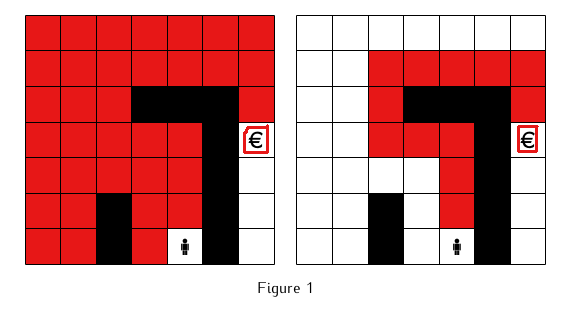
\includegraphics[scale=0.8]{question2.png}

\end{description}